\documentclass[11pt]{article}
\renewcommand{\baselinestretch}{1.8}
\usepackage{textcomp}
\usepackage{fontenc}
\usepackage{graphicx}
\usepackage{float}
\usepackage{caption} % for Fig. captions
\usepackage{gensymb} % for \degree
\usepackage{placeins} % for \images
\usepackage[margin=1in]{geometry} % to set margins
\usepackage{setspace}
\usepackage{lineno}
%\usepackage{cite}
\usepackage{amssymb} % for math symbols
\usepackage{amsmath} % for aligning equations
\usepackage[sort&compress]{natbib}
\bibliographystyle{..//..//refs/styles/newphyto.bst}
\usepackage{xr-hyper}
\externaldocument{reconcilingFLS_main_wbbl}
\externaldocument{newphytrevresp_p2}
\renewcommand{\thetable}{S\arabic{table}}
\renewcommand{\thefigure}{S\arabic{figure}}
% line numbers for letter
% line numbers for letter
\linenumbers
\title{\textit{New Phytologist} Supporting Information}
\date{}
\IfFileExists{upquote.sty}{\usepackage{upquote}}{}
\begin{document}
\maketitle

\noindent \textbf{Article title:} Reconciling competing hypotheses regarding flower-leaf sequences in temperate forests for fundamental and global change biology\\
\noindent \textbf{Authors:} D.M. Buonaiuto, I. Morales-Castilla, E.M. Wolkovich\\

\noindent The following Supporting Information is available for this article:\\

\pagebreak[4]

\section*{Figures}
\begin{figure}[H]
\centering
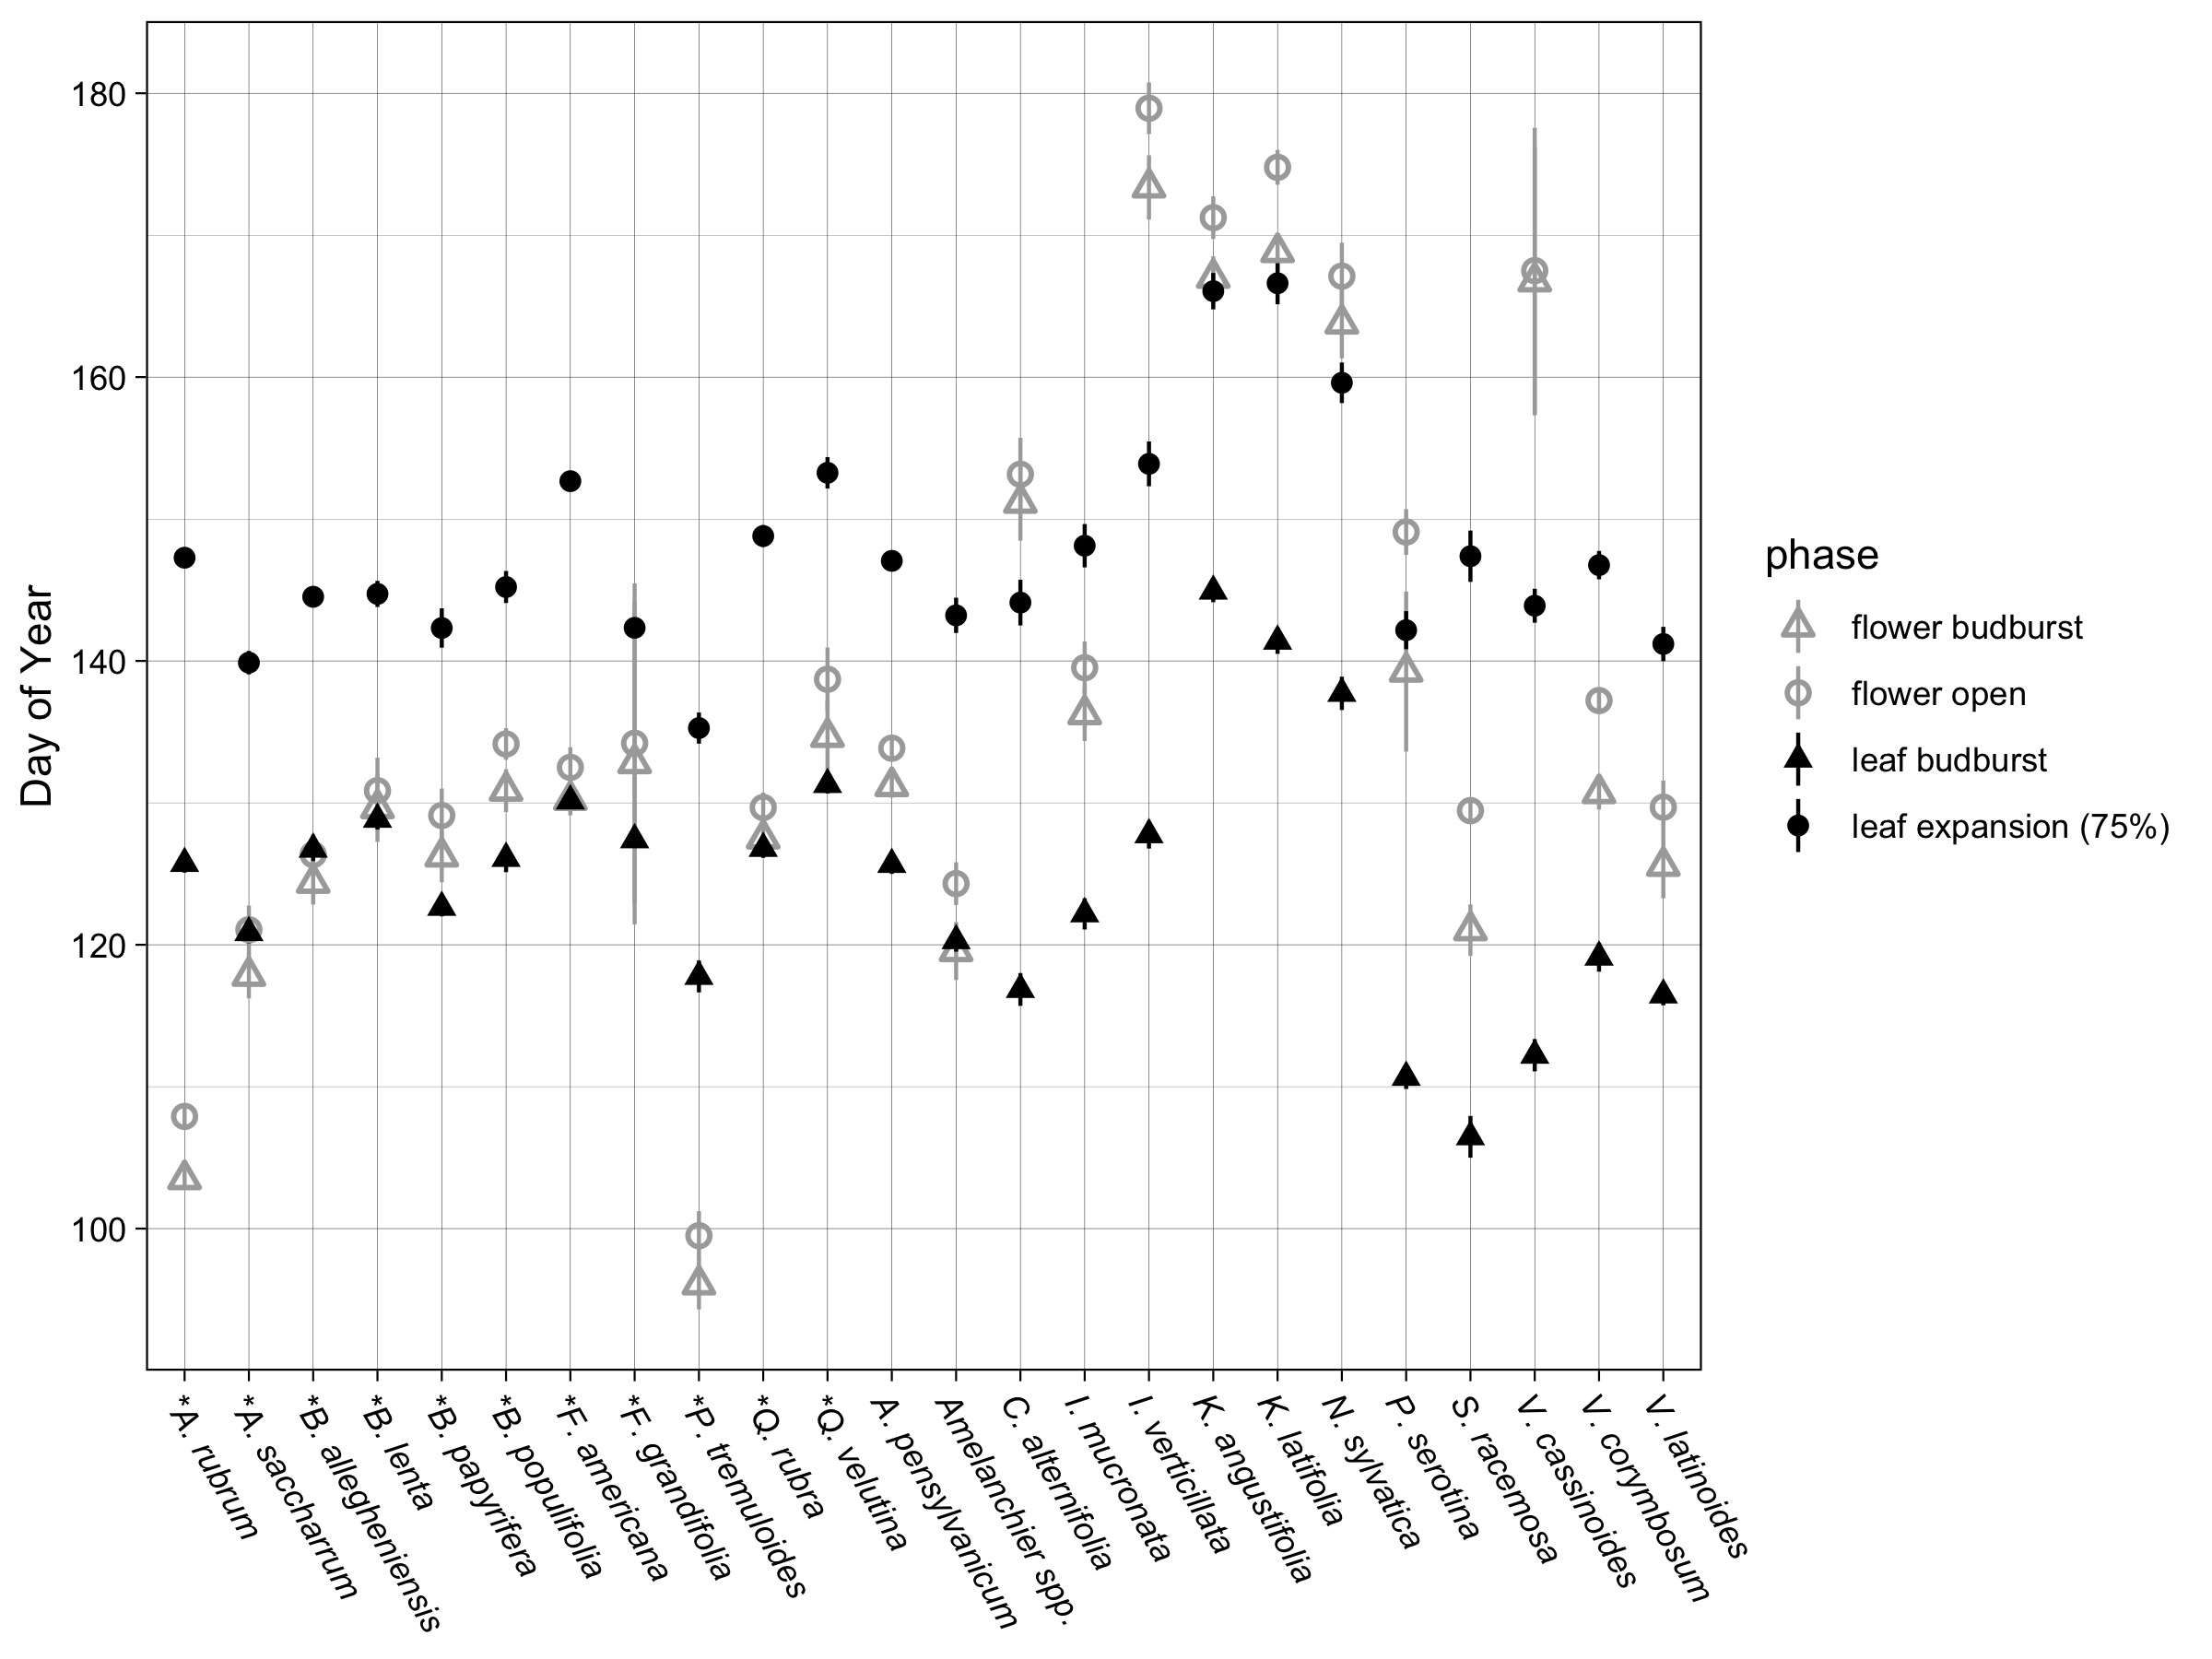
\includegraphics[width=\textwidth]{..//..//HarvardForest/HFmeans_expanded.jpeg} 
\caption{\textbf{Quantitative FLS patterns for woody plants at Harvard Forest in Petersham, MA.} Because phenological sequences consist of several sub-stages it is difficult to unambiguously categorize many species into the current FLS categories. The * accompanying the species name indicates wind-pollinated species.}
\label{fig:HFmeans}
\end{figure}

\begin{figure}[H]
\centering
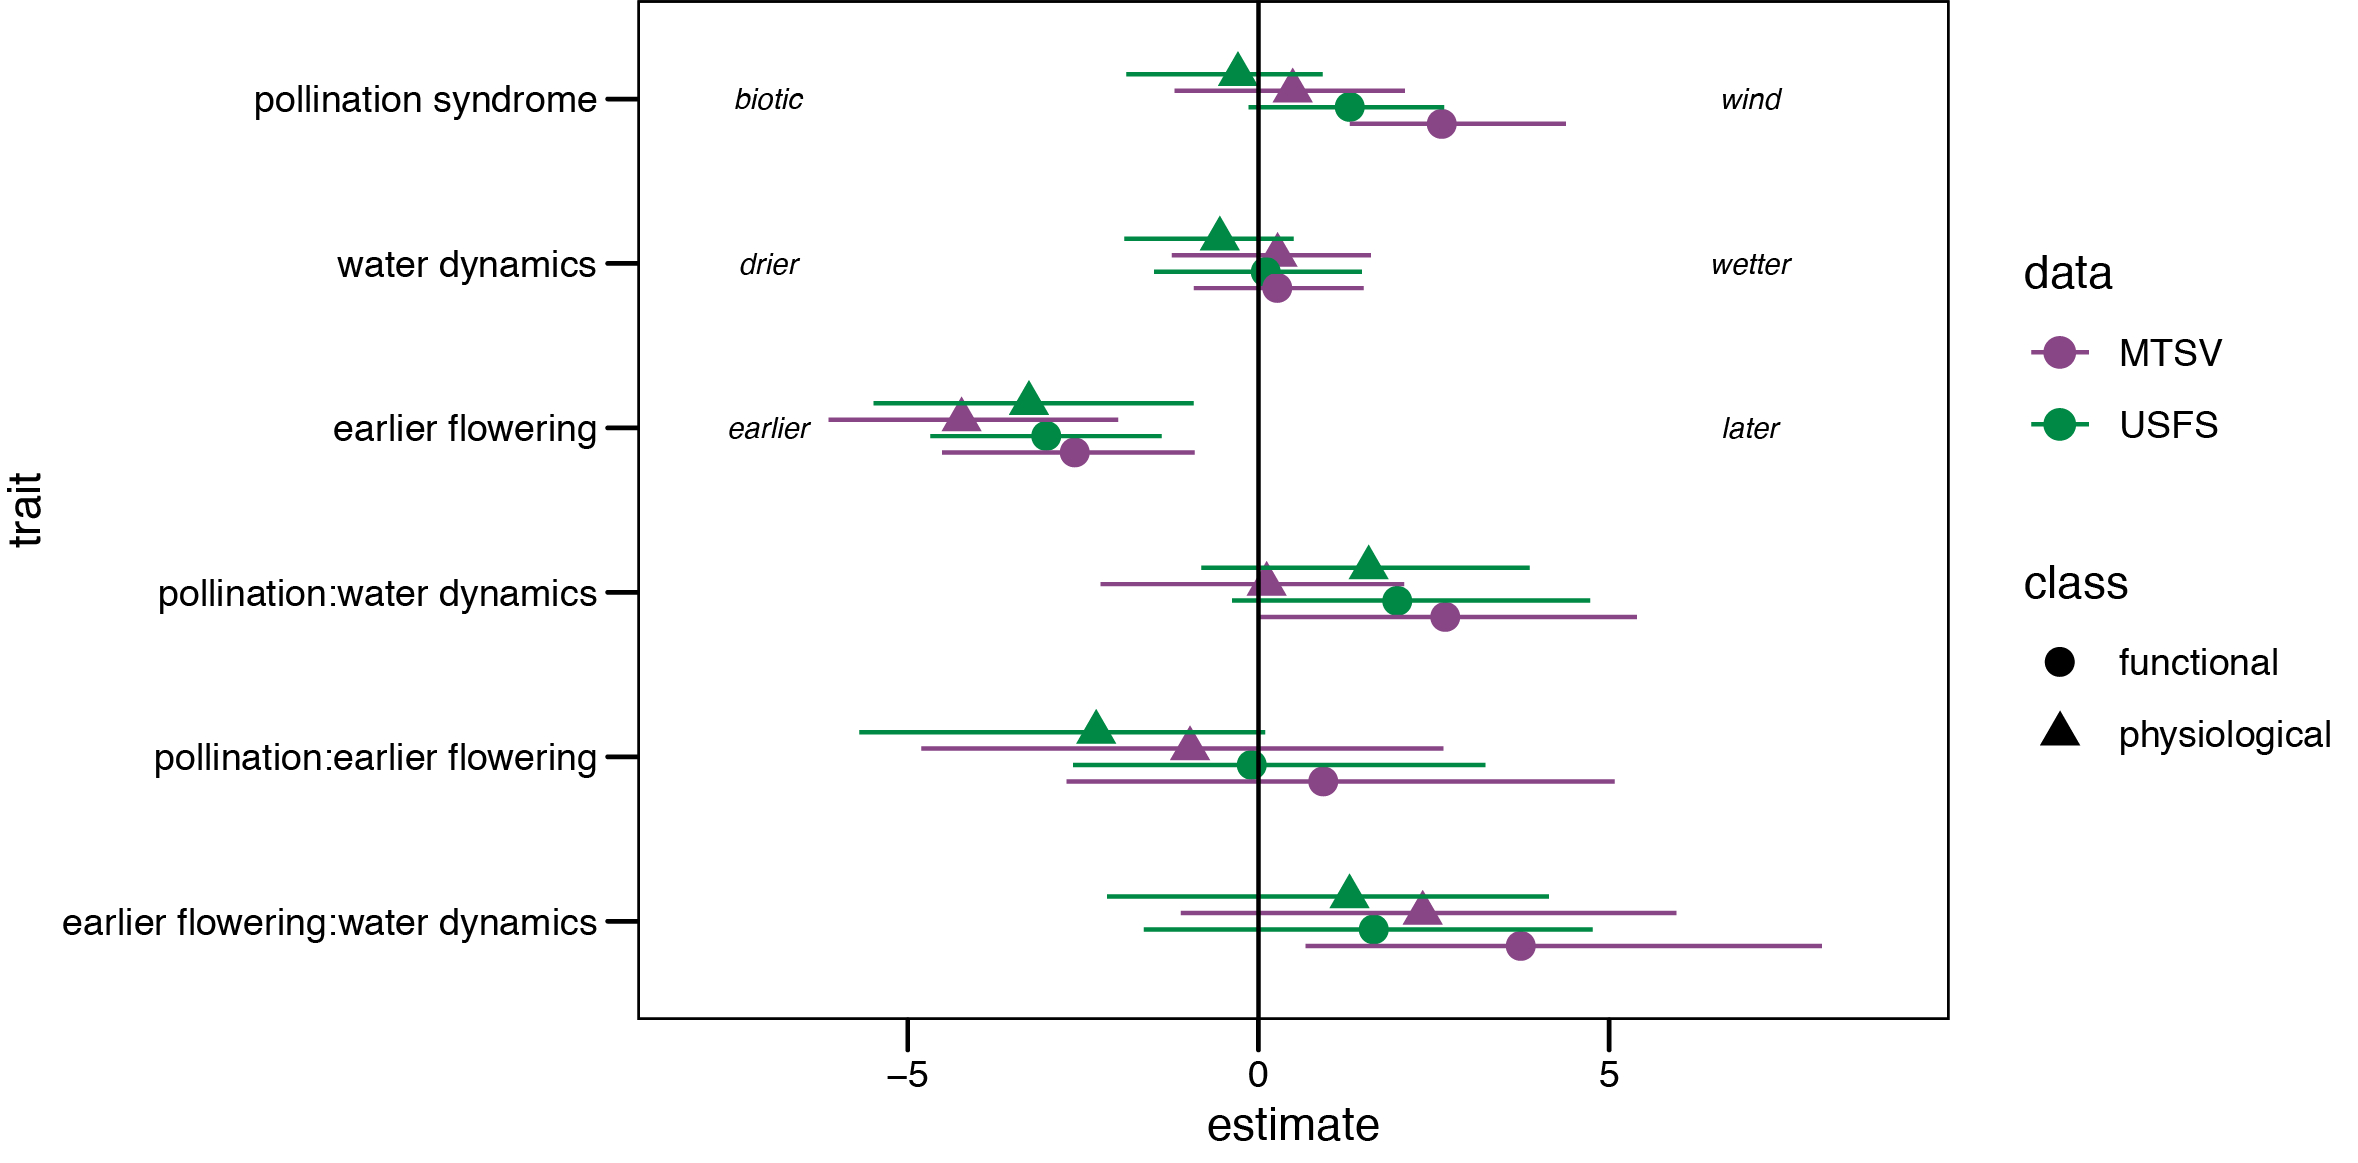
\includegraphics[width=\textwidth]{..//..//MTSV_USFS/MTSV_USFS.png} 
\caption{\textbf{Mean estimates of the effects of FLS predictors on the likelihood a species is hysteranthous vary across datasets and definitions of FLSs.}  We used phylogenetic adjustments and standardized units to make a basic comparison of two datasets (Michigan Trees, Michigan Shrubs and Vines (MTSV) \citep{Barnes2004,Barnes2016} and The United States Forest Service's Silvics Manual (USFS) \citep{Burns1990}) and classes (physiological= no overlap between flowering and leafing, functional= moderate overlap) of FLSs. We chose functional trait predictors related to each of FLS hypothesis. While there is some agreement across models (strong effects of flowering time, no consistent effect interactions between predictors), the effect of other predictors (pollination syndrome, minimum precipitation across species' range) were highly sensitive to how data were defined, potentially biasing any inference from models and compromising the ability to validate the existing FLS hypotheses. Lines represent 95\% bootstrap intervals.}
\label{fig:muplots.USMT}
\end{figure}

\begin{figure}[H]
\centering
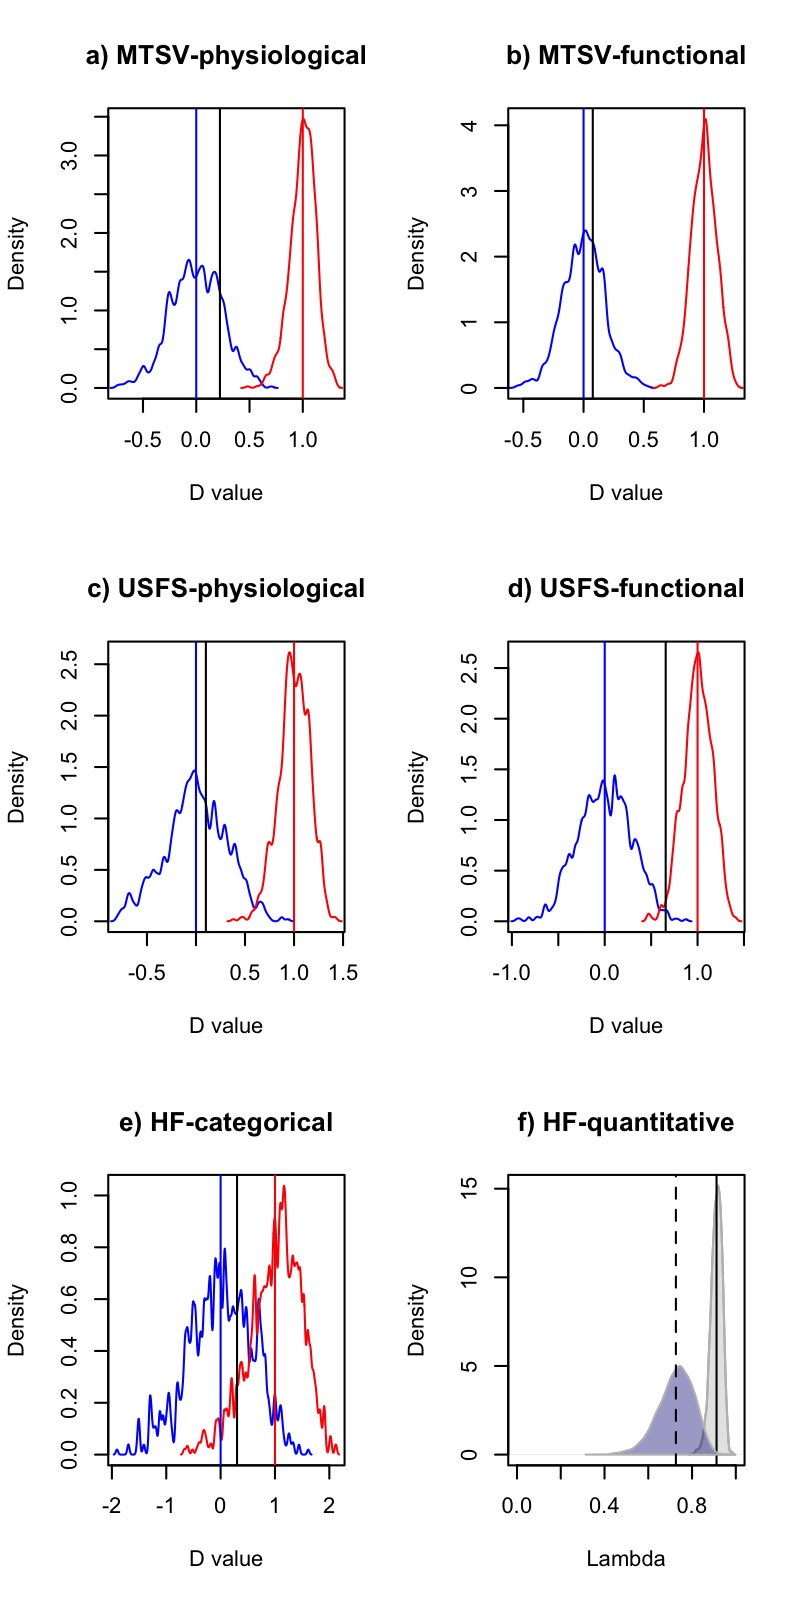
\includegraphics[height=0.8\textheight]{..//..//phylosig.jpeg} 
\caption{\textbf{The phylogenetic signal for FLSs varies between datasets, and is sensitive to how FLS patterns are categorized.} In a)-e),the black vertical line shows the the Fritz's D statistic for binary classifications of FLS estimated from the data, with blue and red lines representing expected D values based on simulations under Brownian threshold model and random model respectively. Panel f) shows the the estimated $\lambda$ values of FLS from the the continuous modeling framework. The solid line indicates the mean estimate of $\lambda$ in the intercept only model and the dashed line indicates the mean estimate of $\lambda$ when all predictors were included in the model. Higher values indicate stronger phylogenetic structure.}
\label{fig:Dstat}
\end{figure}

\begin{figure}[H]
\centering
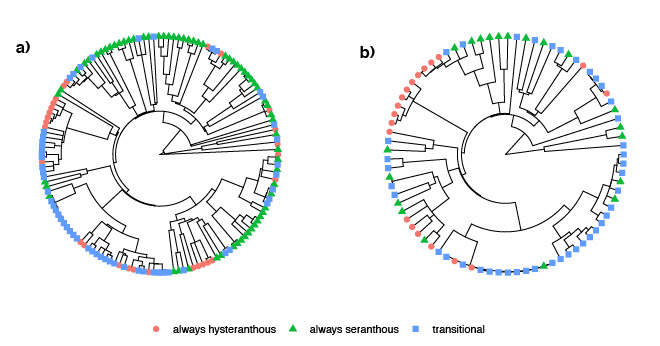
\includegraphics[width=\textwidth]{..//..//cicletrees.jpg} 
\caption{\textbf{Phylogenetic structure of FLSs in MTSV \textbf{a)} and USFS \textbf{b)} varies significantly depending on how FLSs are defined.} Many species are re-assigned to either hysteranthy or seranthy depending on whether FLSs are defined functionally (partial overlap between flowering and leafing allowed) or physiologically (no overlap between flowering and leafing allowed) (blue squares). This modeling choice dramatically alters FLS patterning across the tree, resulting in an unstable phylogenetic signal for this trait.}
\label{fig:phylogeny}
\end{figure}

\begin{figure}[H]
\centering
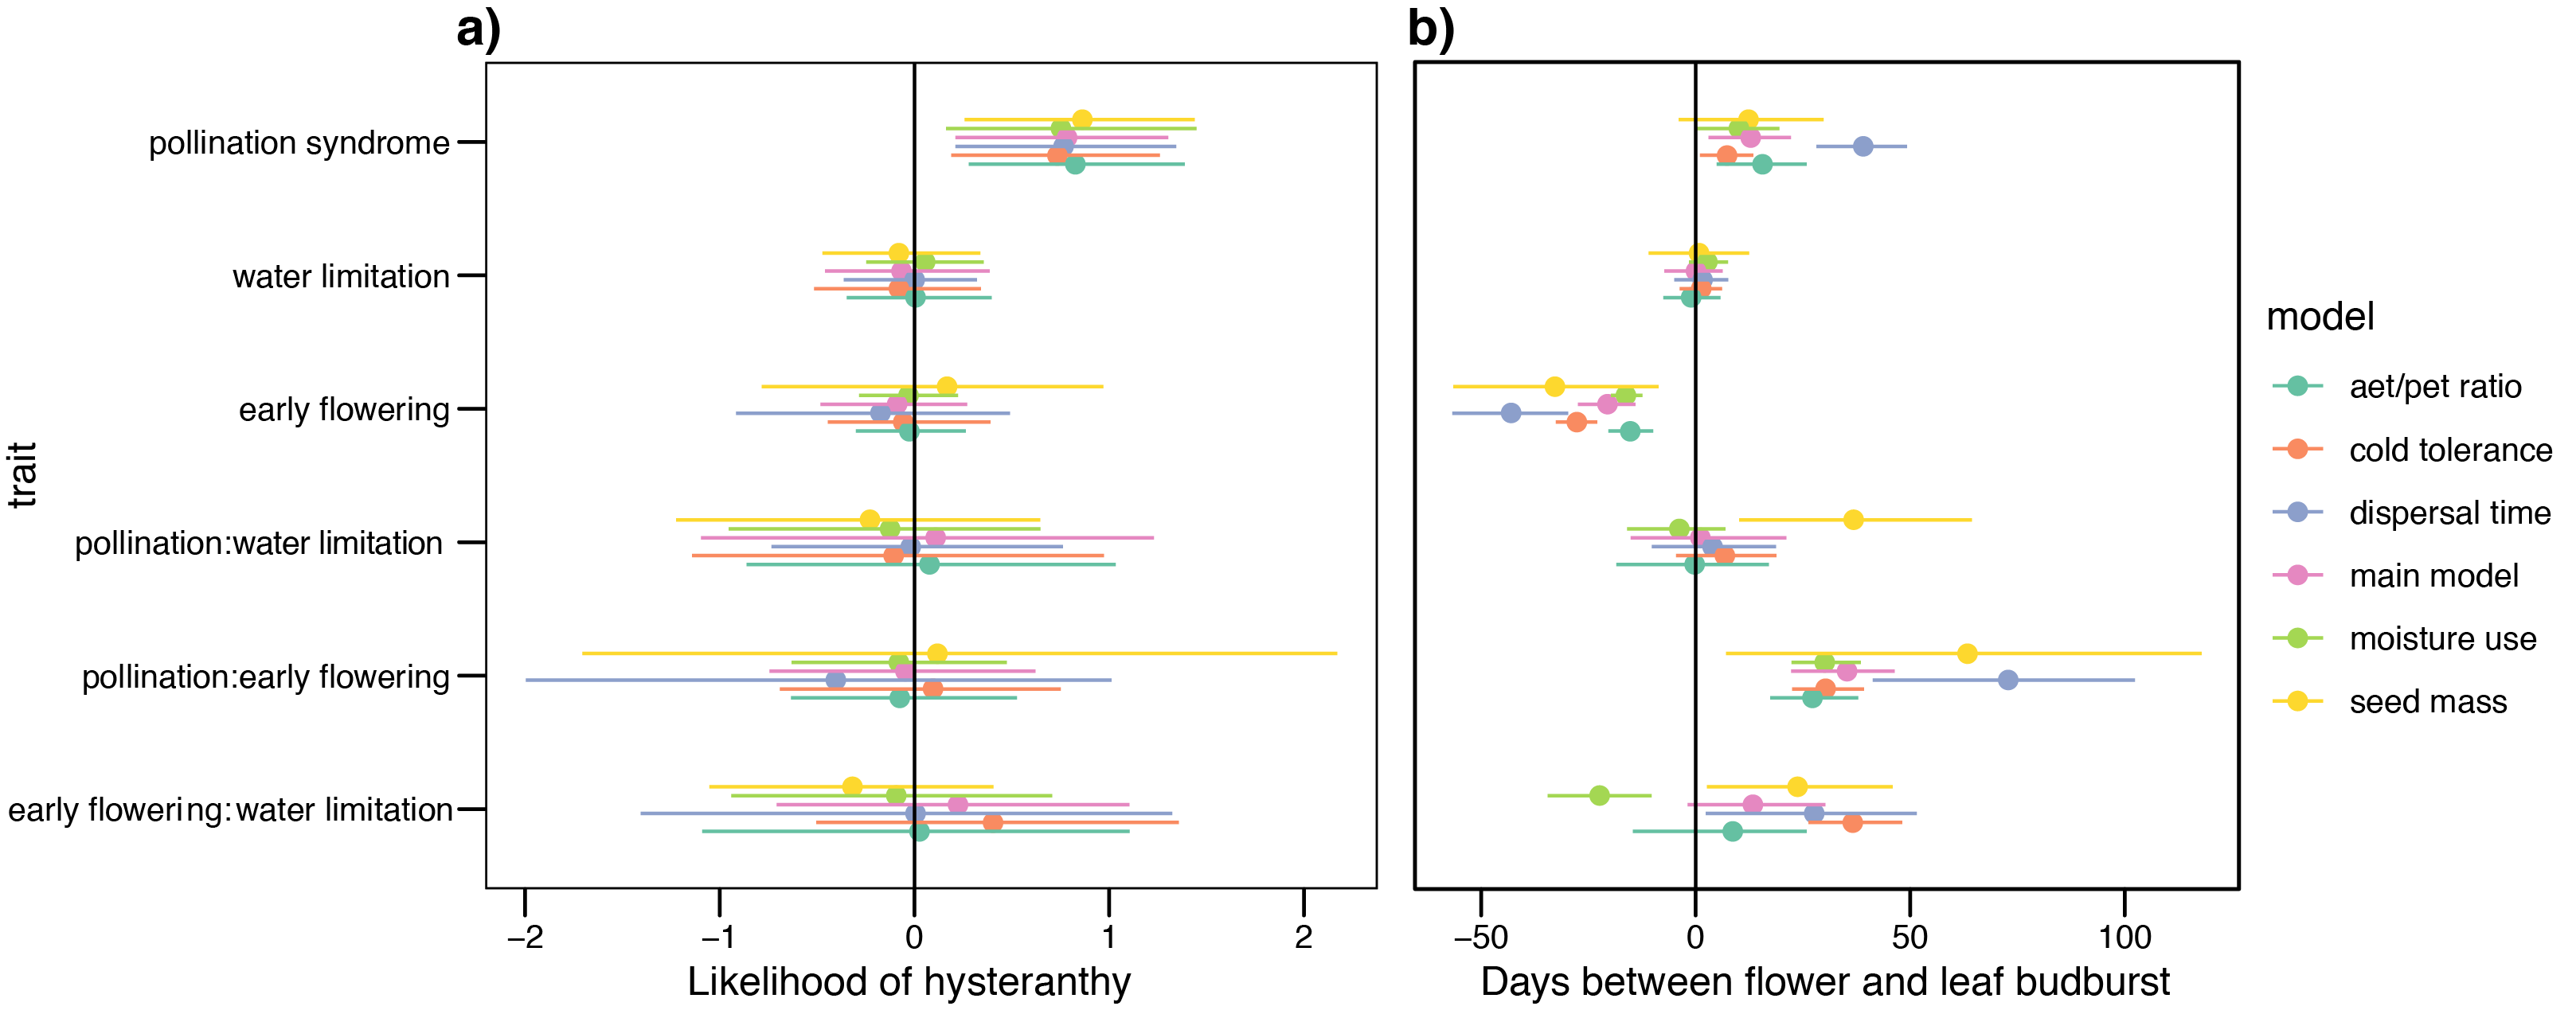
\includegraphics[width=\textwidth]{..//..//alternatepredictors.png} 
\caption{\textbf{Model estimates based on categorical (a) and quantitative (b) FLS data of associations between FLSs and functional traits are stable when alternate traits are used to represent the FLS hypotheses.} In addition to our main model which used minimum precipitation across a species' range to represent the water limitation hypothesis and flowering time to represent the early flowering hypothesis, we ran alternative models with cold tolerancem moisture use and the ratio of actual evapotranspiration to potential evapotranspiration (aet/pet) representing the water limitation hypothesis, and dispersal time and seed mass representing the early flowering hypothesis. Especially for the quantitative model \textbf{(b)}, the exact estimates and uncertainty varied depending on which model we used, but the relative strength among predictors representing each hypothesis remained consistent suggesting the drivers of FLS variation are consistent for the suite of traits that may comprise them. Lines represent 95\% bootstrap intervals.} 
\label{fig:altpreds}
\end{figure}

\begin{figure}[H] 
\centering
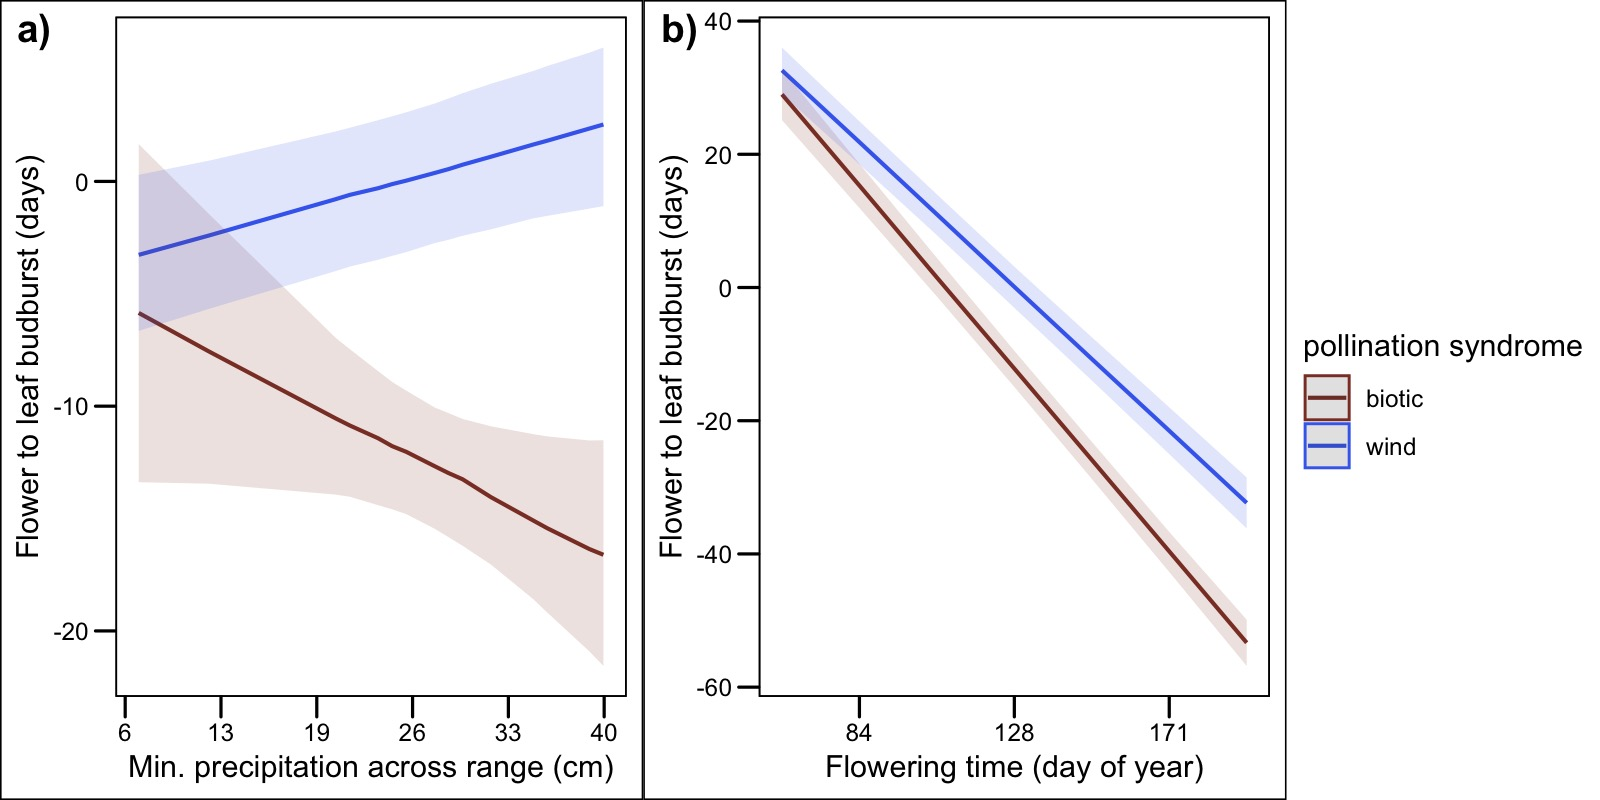
\includegraphics[height=0.4\textheight]{..//..//apcs.jpeg}
\caption{\textbf{Results from a quantitative-hierarchical model accounting for individual variation in FLSs suggests that water limitation may be a driver of hysteranthy in biotically-pollinated but not in wind-pollinated taxa (a)  and that while wind pollinated species tend to always have a longer FLS interphase, the FLSs of bioticly pollinated species are are more sensitive to absolute flowering time (b).} Here we show model-predicted differences in FLSs as a function the minimum precipitation across a species' range and flowering time for a two generic species with contrasting pollination syndromes. Model projections are conditioned on long term phenological data from Harvard Forest in Petersham, MA \citep{OKeefe2015}. The interaction depicted between hydraulic demand and pollination syndrome \textbf{(a)} assumes the mean flowering date (May 8) in the community for both functional types and the interaction between flowering time and pollination syndrome depicted in \textbf{(b)} is based on mean minimum precipitation values for the species included in the analysis (26 cm). Lines and shaded regions indicate mean estimates and 50\% credible intervals respectively. These systematic differences in drivers of FLSs could reflect differences in function of FLSs for wind and biotically-pollinated taxa of temperate forest communities.}
  \label{fig:apcs}
  \end{figure}
  
  \begin{figure}[H]
  \centering
  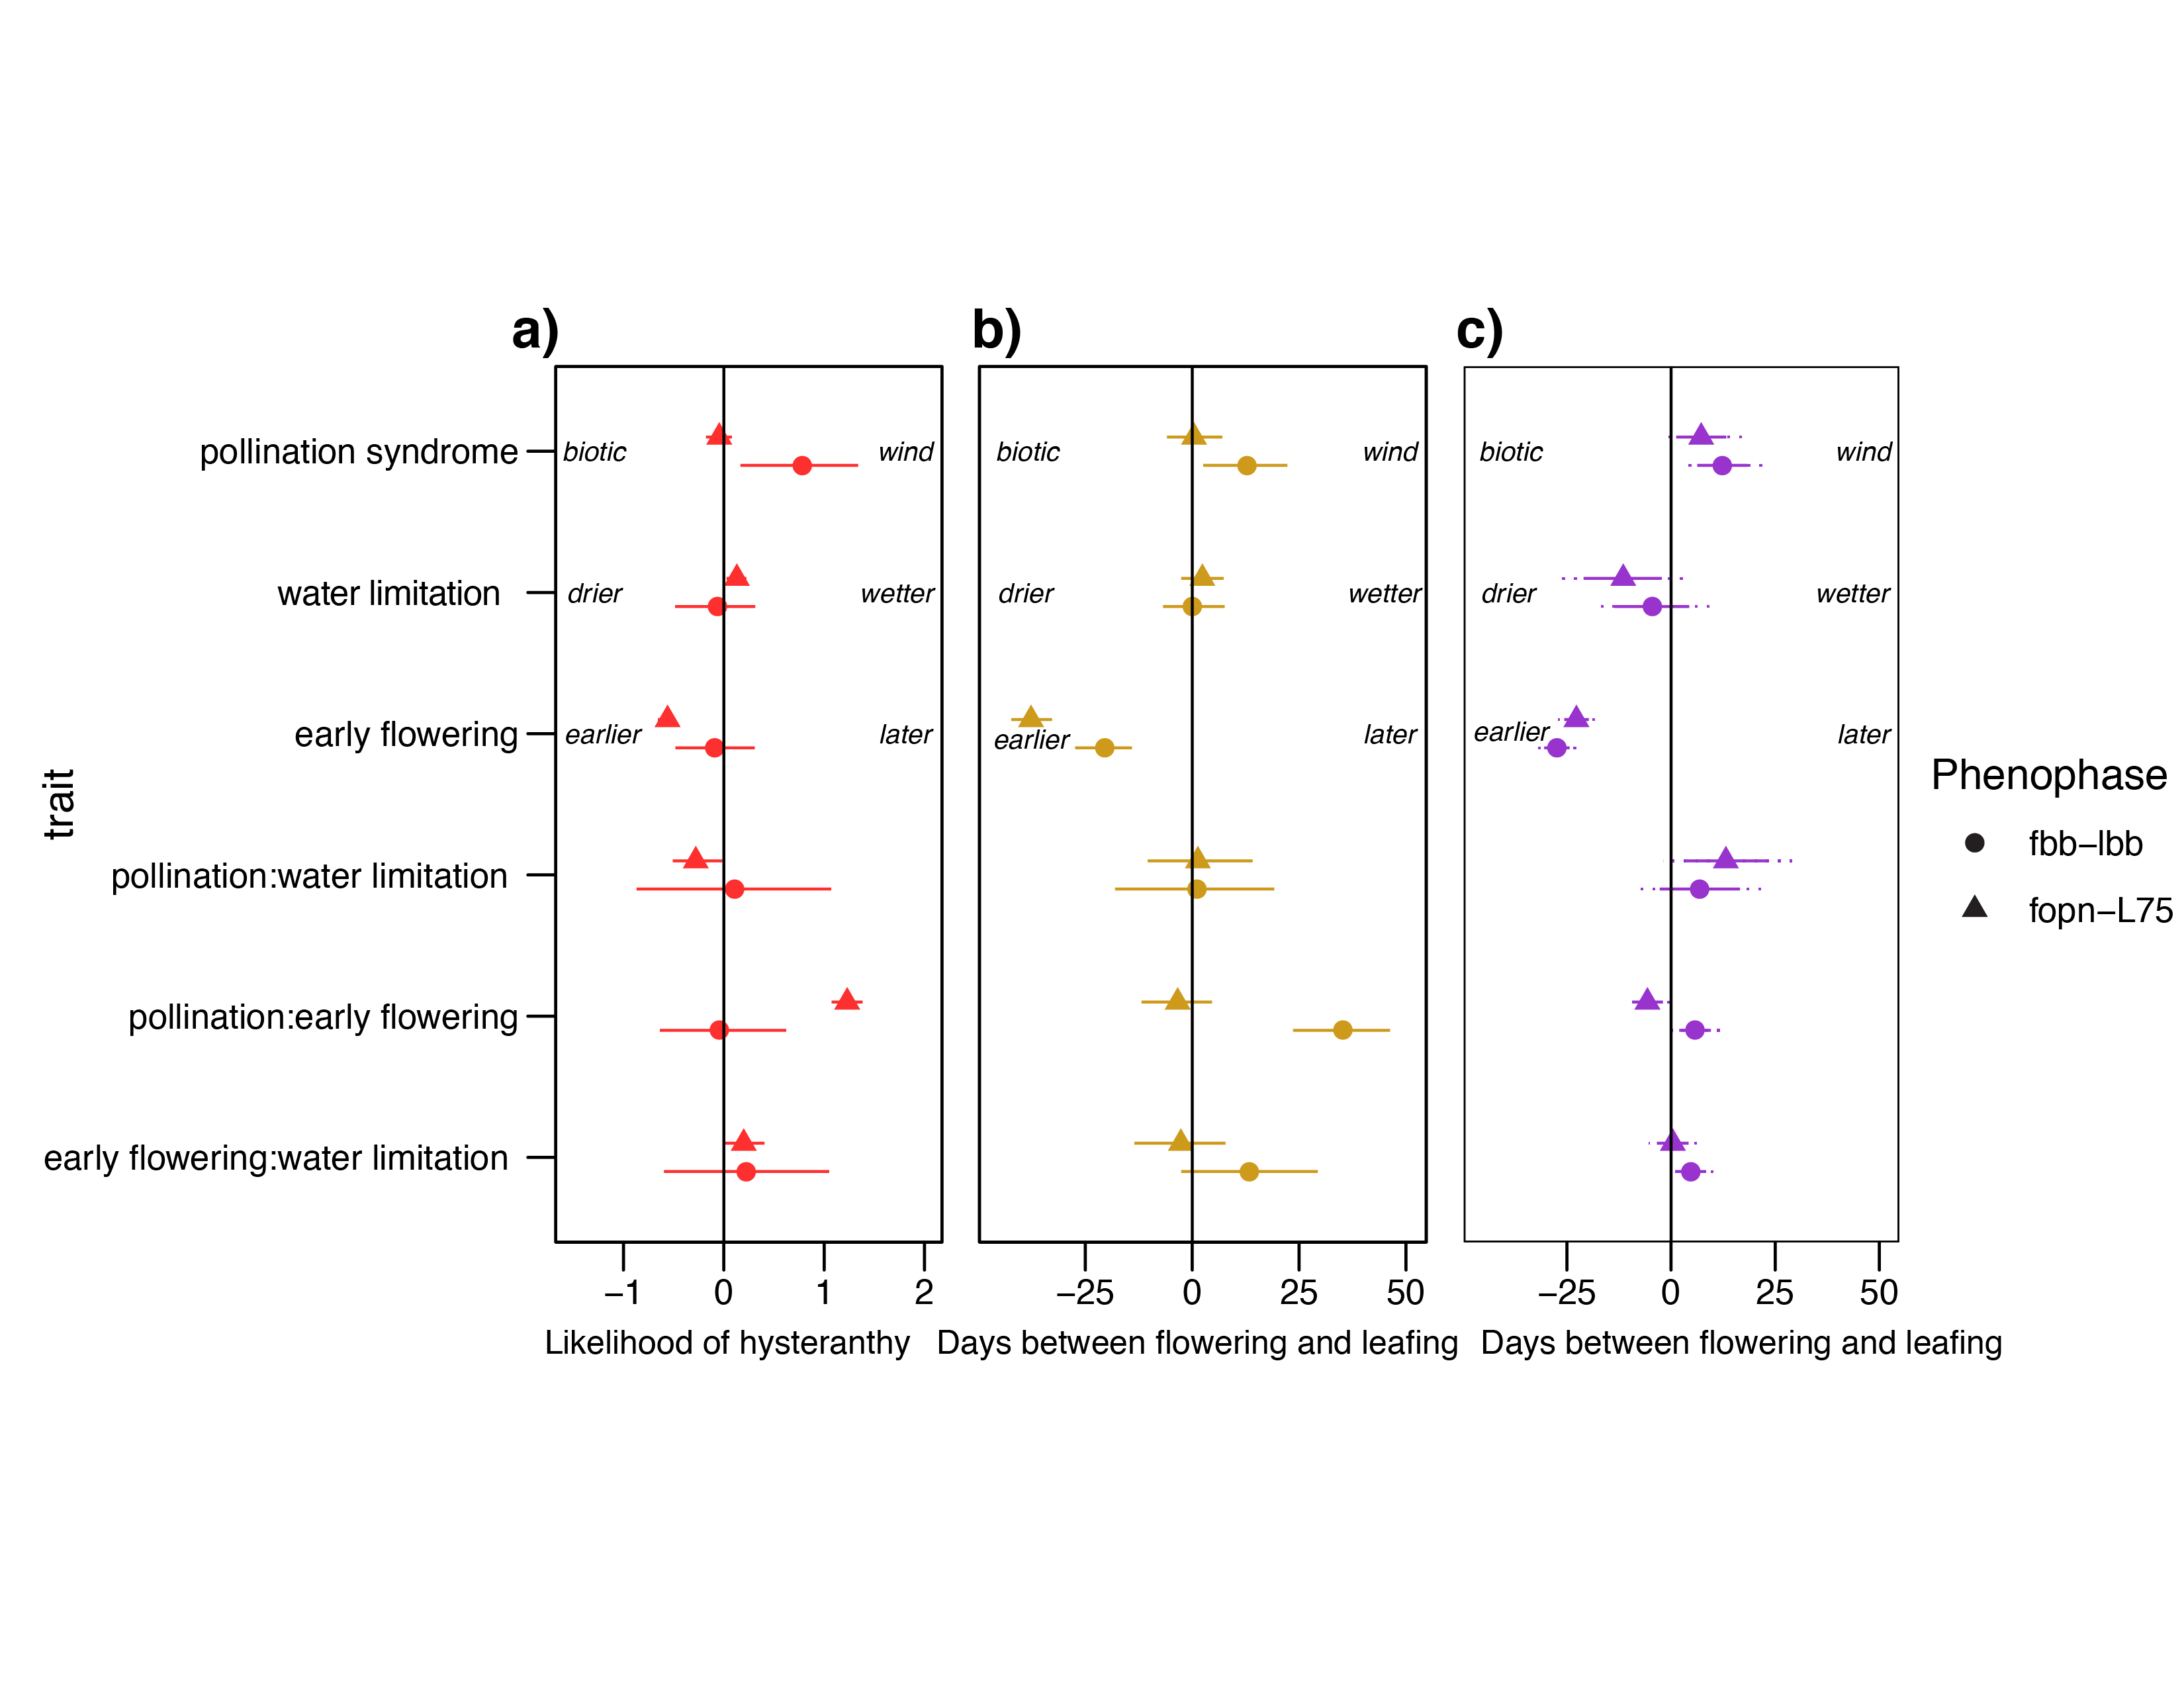
\includegraphics[width=\textwidth]{..//..//HFmodelplots4SUPP-01.png} 
  \caption{\textbf{Comparisons of sensitivity of model estimates to the use of different flower and leaf sub-phases for a categorical  \textbf{(a)}, quantitative (mean trait values), \textbf{(b)} and quantitative hierarchical \textbf{(c)} modeling framework reveal that hierarchical models that explicitly incorporate intra-specific variation may reduce the bias from comparing different sub-phases.} Trait associations vary in strength when FLSs are defined based on different sub-phases of flowering and leafing (e.g. pollinator syndrome in \textbf{(a)}, \textbf{(b)}). The fact that hierarchical models conditioned on intra-specific variation appear to reduce this bias may allow researchers to compare existing FLS data that are not perfectly standardized.}
  \label{fig:sensitivity}
  \end{figure}
  
  \begin{figure}[H]
  \centering
  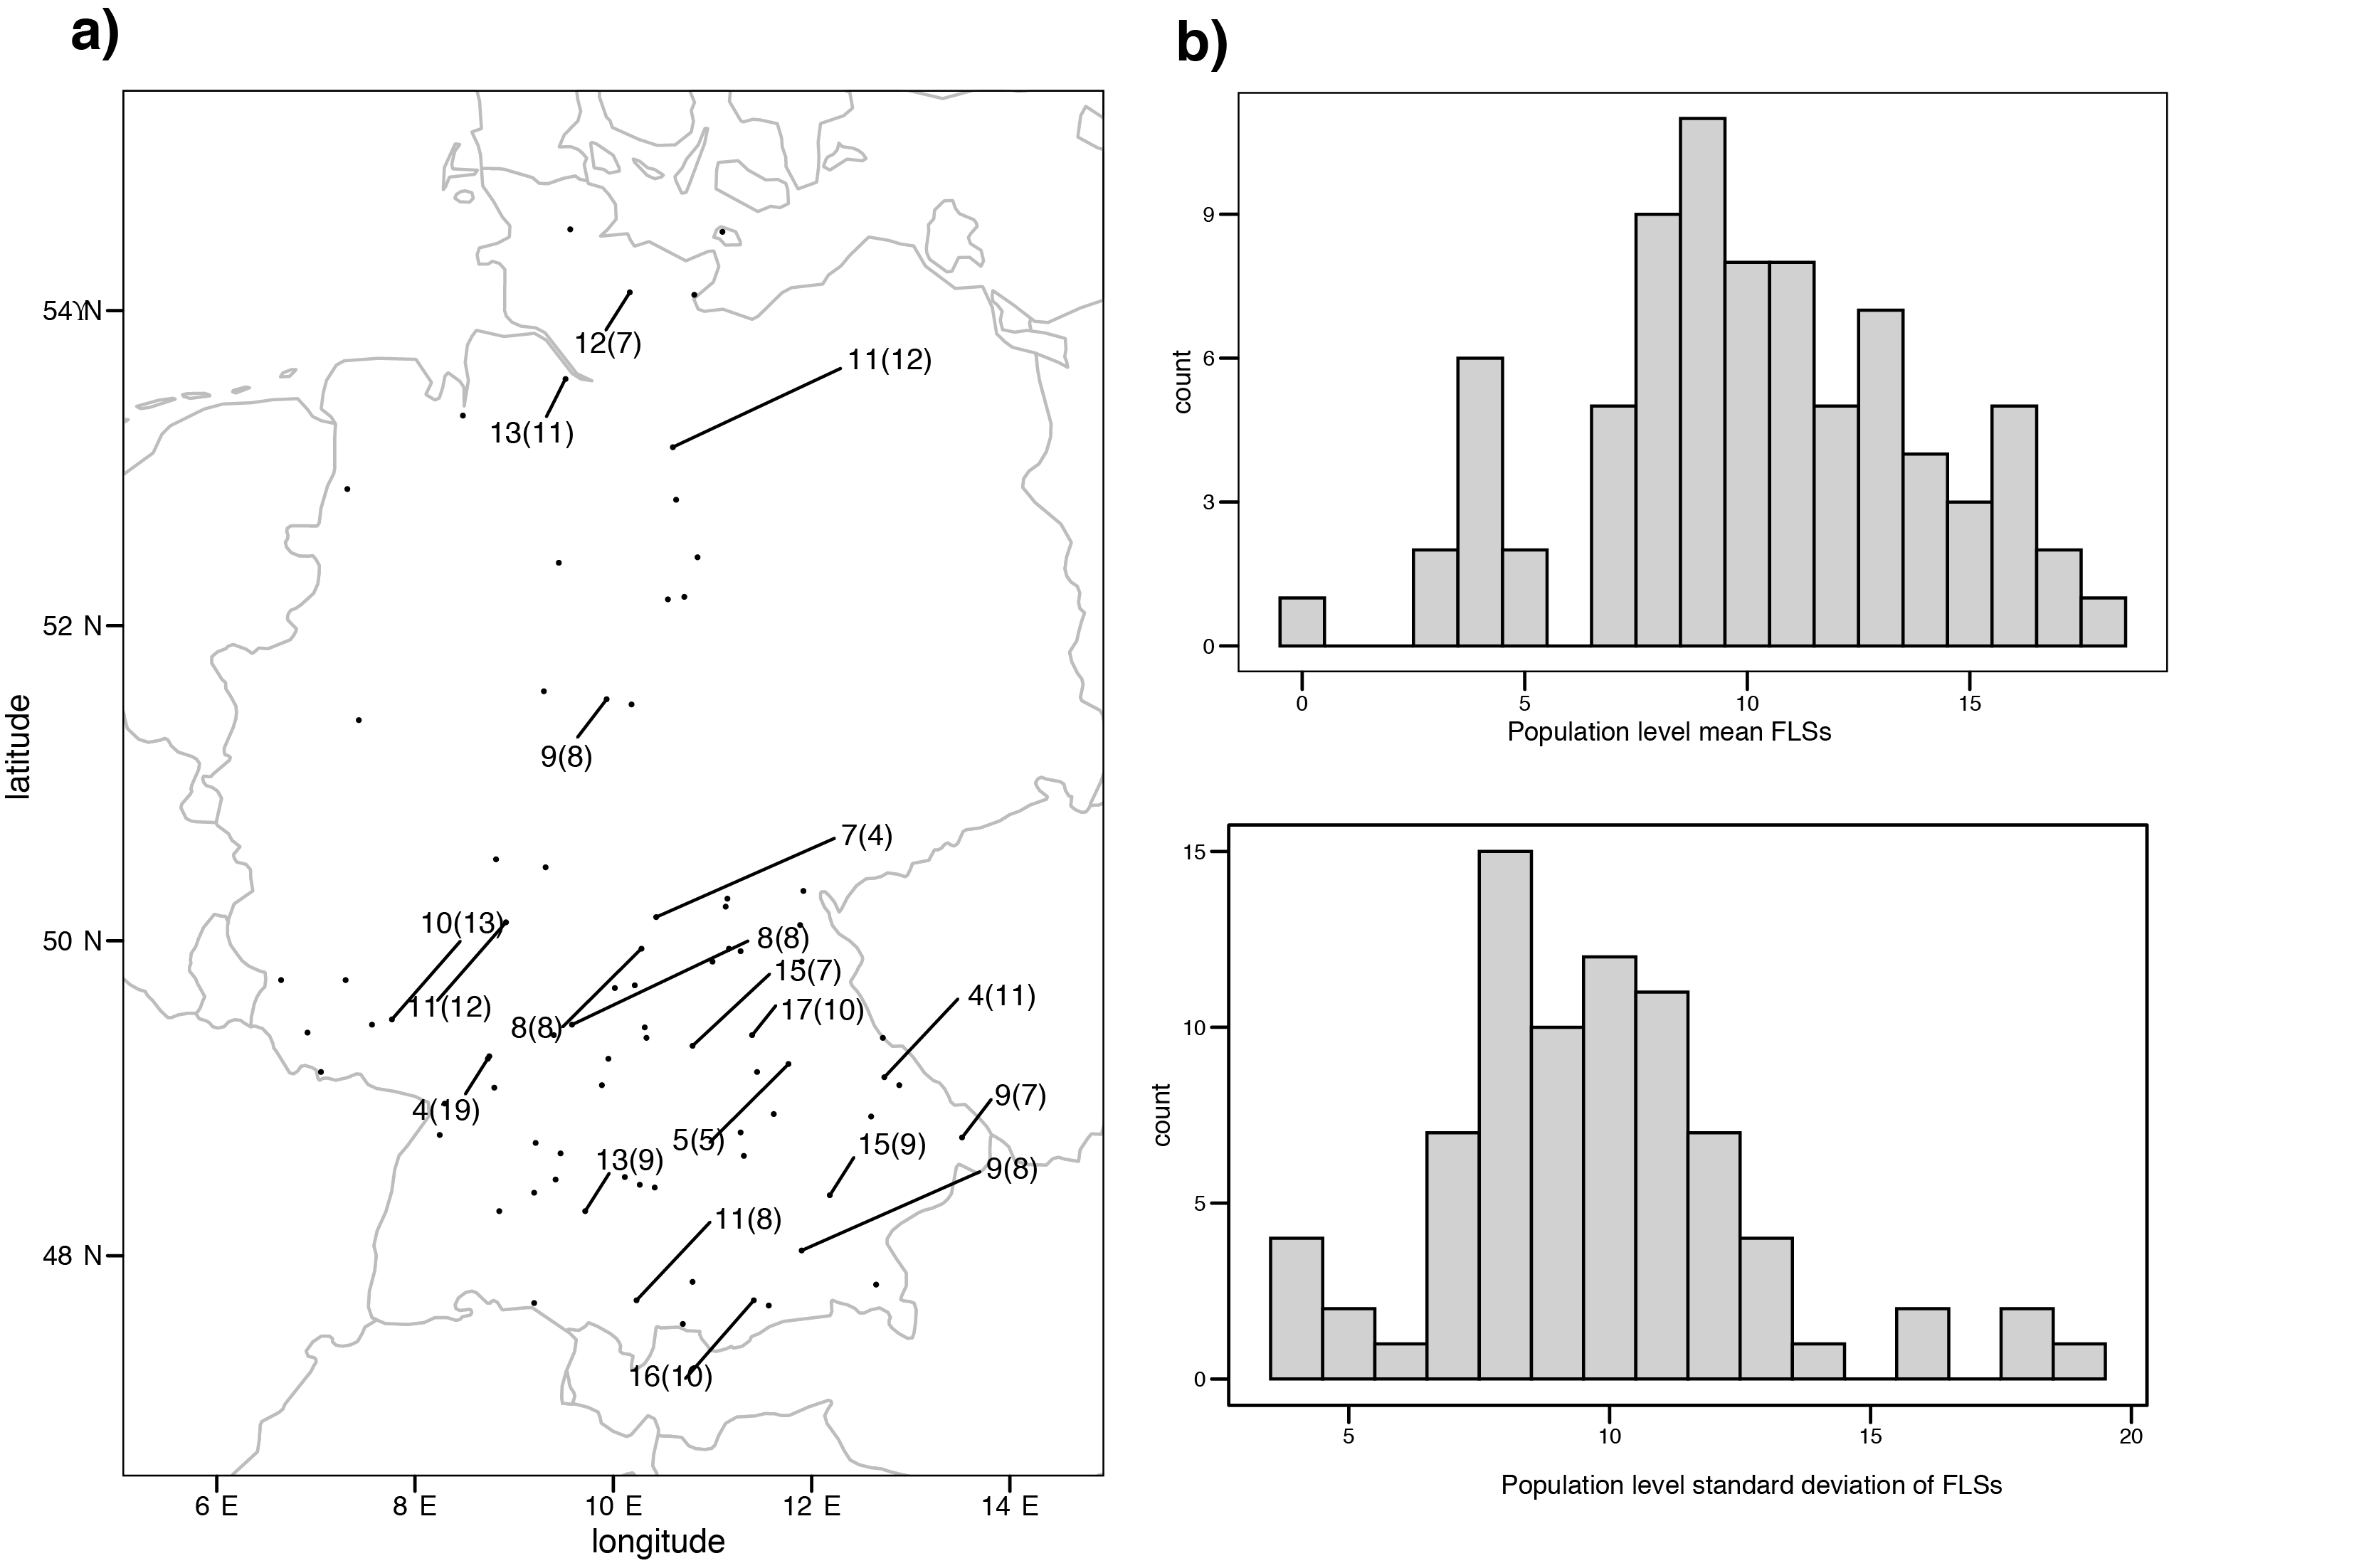
\includegraphics[width=0.9\textwidth]{..//..//popmap.png} 
  \caption{\textbf{FLSs vary significantly among populations of of \emph{Fraxinus excelsior} across Germany}. In \textbf{(a)} each dot represent a population of \emph{F. excelsior} with more than 50 years of phenological observations. We depict the mean and standard deviation (in parentheses) of the days between flowering and leaf expansion for 20 randomly selection populations. In \textbf{(b)}, we show this population level variation for all populations using histograms. Data comes from the PEP725 database \citep{PEP725}. Observations of FLSs at the population level are critical to better understand how environmental conditions shape FLSs and how FLS variation interacts with larger landscape-scale processes.}
  \label{fig:popmap}
  \end{figure}
  
  \pagebreak[4]
  
  \section*{Tables}
  
  \begin{table}[H]
  \centering
  \begin{tabular}{rrr}
  \hline
  HF phenophase & verbal description & approximated BBCH  \\ 
  \hline
  fbb & flower buds first broke with petals visible & 55 \\
  fopn &  50\% of the flower buds were open & 65 \\
  bb &  50\% of the buds were open with visible leaves & 11 \\
  l75 & 50\% of the leaves were developed to 75\% of their final size &  15 \\
  \hline
  \end{tabular}
  \caption{Approximation of phenophases observed in \citep{OKeefe2015} the BBCH scale \citep{Finn2007}} 
  \label{tab:BBCH2HF}
  \end{table}
  
  \pagebreak[4]
  
  \section*{\nameref{Methods S1}}\label{Methods S1}
  
  \subsubsection*{Climate Change and FLS:}
  \noindent To evaluate how FLS patterns have changed over time in association with climate change we obtained phenological data for four European woody plant species with long term phenology records of both flower (BBCH 60) and leafout phenology (BBCH 11) from the Pan European Phenological Database \citep{PEP725}. We restricted the data set to include only stations with more than 50 years of data. Following conventions for modeling effects of climate change, we modeled the number of days between flowering and leafing as a function of time for each species, using a hinge model with 1980 as a break point \citep{IPCC2013,Kharouba2018}. For each species, we display the pre-1980 mean and 95\% credible intervals of the time between flowering and leafing and the post-1980 change in mean time between phenophases that can be attributed to climate change and box plots to summarize the uncertainty in the estimates (Fig. \ref{fig:climchange}).
  
  \subsubsection*{Modeling FLS variation in MTSV and USFS data}
  \noindent For these two categorical, species-level case-studies, we converted verbal descriptions of flower-leaf sequences into a binary response variable. For our more inclusive ``functional" definition of hysteranthy, which allows for some overlap between floral and vegetative phenophases, we included species entries with descriptions \textit{``flowers before the leaves"}, \textit{``flowers before or with leaves"} and \textit{``flowers with leaves"} as hysteranthous. Our more restrictive ``physiological" hysteranthy definition only included species described as \textit{``flowers before the leaves"} as hysteranthous.\\
  
  \noindent For modeling trait associations with FLSs, we chose three predictors to represent the three adaptive FLS hypotheses; pollination syndrome, average flowering time and minimum precipitation across a species' range. We obtained pollination syndrome and average flowering time information directly from the respective data sources and estimates of minimum precipitation across range from the USDA/NRCS Conservation Plants Characteristics (CPC) database \citep{usdancrs}. We coded pollination syndrome as biotic- or wind-pollinated, and assigned known ambophilous species in the genus \textit{Salix} as biotic-pollinated. We re-coded flowering time as the average of the range of months of flowering reported in each data source.\\
  
  \noindent For these case studies, we modeled associations between hysteranthy and the trait predictors with all two-way interactions with logistical regressions in phylogenetic generalized linear modeling framework \citep{Ives2010} using the R package ``phylolm" \citep{Ho2014}. Model results are presented in Fig. \ref{fig:muplots.USMT}. Our models incorporated a published angiosperm phylogenetic tree \citep{Zanne2013} pruned to match the species list for each case study. Species found in the trait data set but not in the original phylogenetic tree were added to the pruned tree at the generic root. In total, 32 species were added to the generic roots for the MTSV data set and eight for the USFS data set. We visualized phylogenetic patterning of FLS across the tree of each case study (Fig. \ref{fig:phylogeny}). The MTSV analysis was based on trait and FLS data for 147 species and the USFS analysis on 81 species. \\
  
  \noindent We ran the models with 599 bootstrapped re-sampling iterations for each data set \citep{Wilcox2010}. We standardized all predictors by subtracting the mean and dividing by two standard deviations to allow for a reasonable comparison of effect sizes between the binary and continuous predictors in this model \citep{Gelman2007}. 
  
  
  \subsubsection*{Harvard Forest models}
  \noindnent From the publicly available Harvard Forest phenology data \citep{OKeefe2015} we calculated the days between flower budburst and leaf budburst for each individual tree per year in the data. We also calculated FLS timing using alternative phenophases; the days between flowers opening and leaves reaching 75\% of their final size. Positive FLS values indicate flowering-first and negative values leafing-first. We transformed these data to compare the inference between categorical, continuous, and intra-specific variation approaches to FLSs. To make the data categorical, we re-coded the continuous FLS measures as binary responses with positive values coded as hysteranthous and negative values as seranthous. For the continuous data, we calculated the mean FLS timing and day of flowering for each species. For the intra-specific variation model, individual variation in FLSs and flowering time was incorporated into the model as a random effect nested within species. These models used the same predictors as the MTSV and USFS datasets (flowering time, pollination syndrome, minimum precipitation across species' range and all two way interactions between predictors). To test the sensitivity of the models to specific functional traits used to represent the FLS hypotheses, we ran additional models based on three alternative functional traits moisture use (defined as the ability to use (i.e., remove) available\linelabel{def} soil moisture relative to other species in the same (or similar) soil moisture availability region" \citep{usdancrs}, minimum temperature across a species range and the actual evapotranspiration/potential evapotranspiration ratio (AET/PET) across a species range for the water limitation hypothesis. We obtained the former two trait values from  CPC and the latter from \citet{Thomspson2012}. Also from the CPC, we obtained data on seed mass (numbers seed/pound) and mean dispersal time (based on estimates from MTSV) as alternative predictors the early flowering hypotheses (see Fig. \ref{fig:altpreds}).\\
  
  \noindent The Harvard Forest analysis included 23 species. While taxonomically limited compared to the MTSV and USFS data, this data set included repeated phenology observations per species over time, and within year variation between individuals per species. \\ 
  
  \noindent For both the categorical and quantitative Harvard Forest models we used a phylogenetic generalized linear modeling framework \citep{Ives2010} using the R package ``phylolm" \citep{Ho2014} built on a Bernoulli probability distribution for the categorical model and a Gaussian distribution for the quantitative model. For the intra-specific variation model, we used a Bayesian phylogenetic mixed modeling framework (PMM) \citep{Garamszegi2014} using the R package ``brms" \citep{Burkner2018}. PMM's incorporate the phylogenetic relationship among species as a random effect, utilizing a variance-covariance matrix based on species relationships to account for the non-independence in the model residuals that can be explained by phylogeny. We also included species as an additional random effect to account for non-independence in the residuals than is not due to phylogeny, and included individual as a nested factor within this random intercept to account for the repeat observations over time and differences among individuals. With this model, we ran 4 chains with 4000 iterations and a warm-up of 3000 iterations each, resulting in 4000 total sampling iterations. Models used weakly informative priors on the intercept and error terms. Increasing priors three-fold did not impact the model estimates. As our primary goal was to directly compare the effects each predictor, we standardized these variables to allow for a reasonable comparison between them {\citep{Gelman2007}. Model results can be found in Fig. \ref{fig:muplotsHF}, Fig. \ref{fig:altpreds}. and Fig. \ref{fig:sensitivity}.\\
  
  %\noindent The three Harvard Forest models are detailed below:\\
  %\begin{enumerate}
  %\item \underline{Categorical model}:\\
  %Pr(y_i &=1) &= logit^{-1} \alpha_{sp[i]} + \alpha_{phylo[i]} + \beta_{pollination syndrome}X_1_[_i_] + \beta_{flowering time}X_2_[_i_] + \beta_{min. precipitation}X_3_[_i_] +\beta_{pollination syndrome}:\beta_{flowering time}X_4_[_i_]+\beta_{pollination syndrome}:\beta_{min. precipitation}X_5_[_i_]+ \beta_{flowering time}:\beta_{min. precipitation}X_6_[_i_] + \epsilon_i\\
  %
  %\epsilon_i & \sim N(0,\sigma^2_y) \\ 
  %
  %\noindent The influence of the phylogeny $\alpha_phylo$ was modeled as follows:\\
  %\alpha_{sp} & \sim N(\mu_{\alpha}, COR[\sigma^2_{phylo}]) \\
  %
  %\noindent THe $\alpha$ for species effects indendent of the phylogeny was modeled as follows:\\
  %\alpha_{sp} & \sim N(\mu_{\alpha}, \sigma^2_{species}) \\
  %
  %\item \underline{Continuous model}: \\
  %y_i &= \alpha_{ind/sp[i]} +\alpha_{phylo[i]} + \beta_{pollination syndrome}X_1_[_i_] + \beta_{flowering time}X_2_[_i_] + \beta_{min. precipitation}X_3_[_i_] +\beta_{pollination syndrome}:\beta_{flowering time}X_4_[_i_]+\beta_{pollination syndrome}:\beta_{min. precipitation}X_5_[_i_]+ \beta_{flowering time}:\beta_{min. precipitation}X_6_[_i_] + \epsilon_i\\
  
  %\epsilon_i & \sim N(0,\sigma^2_y) \\ %I Think this is wrong and should reflect the phyogeny
  %
  %
  %\noindent The effect of the phylogeny was model as above and here, the individual effects within species were modeled:\\
  %\alpha_{ind/sp} & \sim N(\mu_{\alpha}, \sigma^2_{ind/sp}) \\
  
  %\item \underline{Inter-annual model}:\\
  %y_i &= \alpha_{i} + \beta_{annual precipitation}X_1[_i_] + \epsilon_i\\
  %\epsilon_i & \sim N(0,\sigma^2_y) \\
  
  %\end{enumerate}
  \indent To graphically interpret the interactions in the hierarchical model, we calculated the marginal effects using the R-package ``ggeffects" \citep{Ludecke2018}. Fig. \ref{fig:apcs}a shows the water limitation effect of FLS given are based on the mean flowering date (May 8) in the community and  Fig. \ref{fig:apcs}b shows the flowering time effect on FLS based on mean minimum precipitation values for the species included in the analysis (26 cm). \\
  
  \noindent Though we make comparisons between the various HF and MTSV/USFS case studies, differences in data structure between the datasets required us to use alternative modeling frameworks. The categorical, mean quantitative HF data as well as the MTSV and USFS data provide one response variable for each species while the intra-specific variation HF data contains several different response values per species, among individuals and years. The current phylogenetic generalized linear model framework can only fit models with one response value per species, while the phylogenetic mixed model in brms may over-fit models with this kind of data structure and performs better on multi-response per species datasets like HF \citep{BurknerPC}. At the outset, we ran both model types on each case study and while they do yield different absolute estimates, the patterns we found were consistent across each framework, and we report results from the most appropriate model for each dataset.\\
  
  \subsubsection*{Analyses of phylogenetic signals}
  \noindent For all categorical specifications of FLS (MTSV, USFS and HF), we assessed the phylogenetic structure of hysteranthous flowering with Fritz's D-statistic \citep{FRITZ2010} using the ``Caper" package \citep{Orme2013} in R. Fritz's D calculates the sum of changes in estimated node values of a binary trait along edges in a phylogeny and compares this observed value to both a model of phylogenetic randomness and Brownian threshold model. The means of the two data simulations scale values of D to set points of 0 (as phylogenetically conserved) and 1 (random)  \citep{Orme2013}. We visualized the distribution of the traits across the tree for the MTSV and USFS datasets using the R package ``ggtree" \citep{Yu2017}, (see Fig. \ref{fig:phylogeny}). \\
  
  \noindent For the intra-specific variation Harvard Forest model, we estimated the phylogenetic signal for FLS (lambda) directly from the PMM model. To estimate lambda, we fit an intercept-only model with the phylogeny covariance matrix as a random effect and obtained the intra-class correlation value which is the phylogenetic signal. We also estimated the phylogenetic signal from the full model which included all predictors, and in both cases the intra-class correlation in the residuals were high. Estimated phylogenetic signals from all case studies are reported in (Fig. \ref{fig:Dstat}).  
  
  \subsubsection*{The water limitation hypothesis in wet temperate forests}
  \noindent As mentioned, it is surprising that the water-limitation hypothesis for FLS variation might be applicable in temperate regions where water is rarely limited during the main period of reproductive and vegetative phenological activity \citep{Polgar2011}. While recent work found a strong association between drought tolerance traits and FLS variation \citep{Gougherty2018}, this inconsistency suggests that this hypothesis needs further development to be considered in the temperate zone.\\
  
  \noindent There are a number of modifications to the water limitation hypothesis that may explain its relevance to temperate FLSs. This most simple is that hysteranthy in temperate species reflects a ``memory" of an ancestral existence in drier environments and there is no contemporary function relating to plant water status. Hysteranthy may simply be maintained in temperate flora because there is no or weak selection against it. If this is the case, FLS variability should be independent of contemporary water availability. We modified our hierarchical FLS model to test the effect of variation in annual climatic water balance (precipitation - potential evapotranspiration) at Harvard Forest on interannual FLS variation. We calculate water balance from flux tower measurements at Harvard Forest \citep{Hadley2004}, converting latent heat flux to potential evapotranspiration using the R package ``bigleaf'' \citep{Knauer2018}. We found no significant effect of climatic water balance on FLS variation, further suggesting that FLSs variation seems to be independent of water availability in the temperate zone.\\%EMWJune2020 Check your bib file for why the Hadley2004 shows up with extra punctuation

\noindent A second possibility is that the drought tolerance conferred by hysteranthy in the dry tropics has been re-purposed to serve a different function in the temperate zone. Cold\linelabel{watemp3} tolerance, a critical adaptation for life at higher latitudes, may be conferred by many of the same physiological adaptations as for drought tolerance in dry regions \citep{Zanne2013}. For the species in our analyses, we found a strong correlation (0.85) between minimum precipitation and temperature across species' ranges. It is possible that hysteranthy is among the suite of traits that allowed dry-adapted taxa to move into colder temperate regions. Association between hysteranthy and cold adaptation have been found in some families \citep{Gougherty2018}. Though the mechanism by which hysteranthous flowering may contribute to cold tolerance has not been thoroughly investigated, this correlation remains a promising avenue for applying\linelabel{wat2} the water limitation hypothesis in the temperate zone.\\

\clearpage

\bibliography{..//..//refs/hyst_outline.bib}


\end{document}

